\section{Where the argument is
weakest}\label{where-the-argument-is-weakest}

I distinguish overstated implications from numerical mistakes. The brief
already acknowledges several limitations: material-only hardware
savings, use value rather than net benefit for the Protein Data Bank
(PDB), the sponsored venture study, convergence rather than a blanket
closing trend, and young AI-tool cohorts. Those corrections deserve
credit. The remaining problem is that the recommendations often behave
as if those caveats do not constrain the investment conclusion.
\citep{InputBrief,InputRecommendations}

\subsection{Public value is repeatedly substituted for shareholder
value}\label{public-value-is-repeatedly-substituted-for-shareholder-value}

\textbf{Brief claims 1, 2, 3 and 5; pattern 1; proposal IP rationale.}
The USD 8.8 trillion estimate is the hypothetical replacement cost to
user firms if each had to rebuild widely used open-source software. It
is not revenue, willingness to pay, an addressable market, or a cash
flow belonging to an open-source supplier. The USD 4.15 billion estimate
is the cost to recreate the sampled widely used software once, not a
price for all open software. The original authors explicitly describe
this replacement-value construction. \citep{Hoffmann2024Value}

The USD 374 billion aggregate in this export for 33 commercial software
entities does approximately reproduce the brief's USD 375 billion. But
comparing mixed-date market capitalizations, acquisition prices and
private marks with an economy-wide replacement-cost estimate is not a
capture-rate calculation. Databricks alone contributes \textbf{50.8\%}
of that software total; the top three contribute \textbf{66.1\%}. These
examples prove that some businesses commercialize open ecosystems, not
that releasing an alloy lab's methods maximizes its equity value.
\citep{InputData}

The PDB's reported 800x use/cost and 160x R\&D-return/cost figures do
not establish incremental net benefits caused by openness, still less
returns to a private provider. I cannot re-audit that calculation from
these attachments because its underlying source files are missing. The
NIH result is stronger evidence: the primary paper reports 12-27\% more
in-text patent citations after its access mandate. But the treatment is
access to biomedical articles, and the outcome is citations, not patent
quality, alloy qualification, revenue, or investor returns. The reader
cannot transfer that causal estimate to open hardware or open
compositions. \citep{Bryan2021}

\subsection{The headline venture study does not establish a causal
openness
premium}\label{the-headline-venture-study-does-not-establish-a-causal-openness-premium}

\textbf{Brief claim 6; recommendation 4.} The Linux
Foundation/Serena/COSSA study reports USD 1.3 billion versus USD 171
million at IPO and USD 482 million versus USD 34 million at acquisition.
Its own definition includes accessible code, open weights and mixed
proprietary products, not just permissively licensed firms. Its methods
describe more than 800 VC-backed companies and normalization by founding
year, geography and sector. Those are useful comparisons, not randomized
treatments. \citep[pp.~8--9, 39--41]{Boysel2025State}

The headline medians condition on successful IPO or acquisition. They do
not multiply the probability of success by net proceeds after dilution,
liquidation preferences and capital invested, or account for losses on
failures. Founder quality, market attractiveness, prior traction and
investor selection remain plausible explanations. The report's IPO
capital-efficiency slope difference is \textbf{not statistically
significant (p=0.2134)}; it reports an acquisition-slope difference
(p=0.0001). It is not fair to dismiss the whole study as sponsorship,
but it is equally unfair to sell its exit medians as an unconditional
expected-return advantage.

There is also a reproducibility warning: page 39 literally says its exit
comparison uses US infrastructure companies ``founded after 2018,''
while page 8 describes 2000-2024 data and page 39 gives an eight-year
median time to IPO for COSS. Those statements cannot all describe that
filtered sample as written. It may be a typo; I would require the cohort
definition and underlying denominators before relying on the headline.
\citep{Boysel2025State}

\subsection{``87\% cheaper'' is not a fully burdened
autonomous-laboratory cost
comparison}\label{cheaper-is-not-a-fully-burdened-autonomous-laboratory-cost-comparison}

\textbf{Brief claim 4; recommendations 1 and 4.} The Pearce review
processes 119 published designs and records material costs and available
proprietary comparators. It acknowledges fabrication skill, quality
assurance and reliability challenges. \citep{Pearce2020} Published
successful designs, incomplete comparators and self-fabrication costs
are not representative of industrial installed cost.

Engineering, calibration, validation, uptime, spares, support, safety,
warranty and integration labor belong in the denominator. A USD
100-2,000 demonstration device and a USD 1 million specialized
industrial system are not substitutes merely because both are called
self-driving laboratories. The reported USD 2.24 profit on an USD 80 kit
is \textbf{2.8\%} of price and apparently not an audited, fully burdened
margin. It is a warning about that kit, not evidence that all hardware
sales fail or that services will work. The labor-intensive alternative
could be worse.

\subsection{``Already fits the winning pattern'' is the most
investment-relevant
overstatement}\label{already-fits-the-winning-pattern-is-the-most-investment-relevant-overstatement}

\textbf{Brief final pattern; recommendations 1 and 4.} Open
orchestration on closed instruments is an architecture, not a validated
business model. Only about 4 of 20 instruments reportedly have
programmable interfaces; the supplied supporting audit is absent.
Accepting that estimate implies an integration bottleneck, not a moat.
The export has only eight usable multiples across the broad
hardware/science analogues in groups D-G, and just four in group E
itself.

The documents conflate three quite different investees: an automation
software supplier, an operator selling lab services, and a materials-IP
company licensing qualified alloys. Their costs, gross margins,
defensibility, capital requirements and acquirers differ. The lab needs
to choose a paying customer and a scarce deliverable before choosing an
openness narrative.

\subsection{Foundation durability, fork activity and founder status are
not equity
evidence}\label{foundation-durability-fork-activity-and-founder-status-are-not-equity-evidence}

\textbf{Brief claims 7 and 8; recommendations 2 and 7.} Eight
deliberately selected, well-known surviving forks are not a denominator
of all forks. Commit counts are not equivalent to maintenance quality,
paying deployments or shareholder outcomes. A fork's success can
preserve the public good while weakening the original vendor's
bargaining power.

Neutral governance may credibly prevent a vendor from withdrawing
rights. That is valuable to users but can limit a spin-out's exclusive
control and saleability. In this rubric, level 4 partly \emph{means}
neutral/open governance; using its association with continued openness
as independent validation risks circular reasoning. Grants and
institutional mandates also change survival incentives. ``The university
belongs to the category that stayed open'' does not imply that a
VC-financed spin-out should inherit the same objective function.

The recommendation that \textbf{10 of 15 closing moves came at or after
acquisition is not reproducible from the supplied event coding under a
straightforward historical definition}. I find 15 closing rows at
organizations with a recorded acquisition or take-private, one undated;
\textbf{7 of 14 dated rows} are at or after the first such event year
(one is same-year). Restricting instead to currently acquired
organizations gives 6 of 11. Cloudera's restriction began in 2019 before
its 2021 take-private, although full implementation was in 2021;
Docker's 2019 acquisition row concerns a business sale rather than a
clean whole-company exit. Different interpretations are possible, but
none of this is evidence that acquisition \emph{caused} closing.
\citep{InputData}

\subsection{The AI-era and open-science measures are not
commensurate}\label{the-ai-era-and-open-science-measures-are-not-commensurate}

\textbf{Brief claims 9-11 and added AI-tool cohort.} Open articles, open
weights, unrestricted commercial weights, source code, data and
governance are different rights. Averaging their scores does not create
a common economic treatment. Group I contains \textbf{19 releases in
this export}, not the brief's earlier 17-release reference; the same
corporate parents also appear elsewhere. The 2.84 mean current release
score is therefore not 19 independent companies' openness choices.

No SSPL/BSL transitions in a young 17-company AI-tool cohort cannot
answer what happens after commercialization pressure arrives. ``Seven
exits'' includes mergers and undisclosed or partial combinations, not
seven known profitable exits. A 50x ratio of maximum training runs is
unstable and does not measure the economics of physical experiments.
Text mentioning science more frequently is marketing evidence, not a
signed purchasing commitment. These observations may motivate further
study; they do not support a return premium.

\subsection{The proposal makes potentially irreversible commitments
before validating the
business}\label{the-proposal-makes-potentially-irreversible-commitments-before-validating-the-business}

\textbf{Recommendations 3, 7 and 8; suggested proposal language.}
Publishing all failed runs, composition data and methods while saying
that services and data capture value leaves unanswered what data remain
scarce and why customers cannot obtain the same result from competitors.
A 12-month release clock is not a moat if industrial qualification and
selling cycles exceed it. A named prospective licensee at Month 6 is an
arbitrary commercial gate without demonstrated customer timing; absence
of a licensee then does not imply absence of valuable future IP.

I would not treat ``as the award terms allow'' as legal clearance. The
actual solicitation, award, university ownership rules and third-party
licenses need counsel's review. A thin adapter does not automatically
cure SDK restrictions. Derived CALPHAD results are not automatically
redistributable merely because raw databases are withheld. A provisional
filing is neither an issued patent nor freedom to operate.
Public-by-default GitHub records can disclose inventions, customer
information or operational attack surfaces. \citep{InputProposal}

\textbf{What I would keep:} negotiate API, export and driver-publication
rights before buying instruments; clarify university ownership; maintain
attribution and license compliance; define a data schema; and budget for
critical dependencies. These reduce operational risk regardless of
whether openness commands a valuation premium. The recommendations to
release everything, rule out units and call the architecture a winning
pattern do not follow from the evidence.

\section{What the dataset actually
says}\label{what-the-dataset-actually-says}

\subsection{Denominators and methods}\label{denominators-and-methods}

I use the supplied 179-row master and 223-row event export. There is no
duplication by slug, but there are composite units
(Cloudera/Hortonworks; MySQL/Sun; vLLM/Inferact), projects, foundations,
model releases and corporate science programs. Thirteen event rows lack
a year. The company export omits the underlying case JSON's source URLs
and field-level provenance; I can reproduce the calculations, not
certify all inputs. \citep{InputData,InputSchema}

My primary commercial sample is \textbf{118 non-model entities} with an
explicit status of public, private VC, private bootstrapped, private PE,
acquired or defunct. I do not silently classify unknown organizations as
failed or closed. I exclude all 19 model-release rows and statuses
indicating public goods/noncommercial ownership. The 17 unknown-status
rows remain visible in the audit. An expanded, category-based sample has
133 rows and yields the same 37 financial multiples, although event
denominators change. This is a unit-of-analysis choice, not a claim that
nonprofits create no value.

Only positive amounts explicitly labeled \textbf{market cap, private
valuation or acquisition price} enter reported company value. Seven
positive \texttt{latest\_value\_usd} entries instead describe annual
revenue, grants or awards: Apache, HDF Group, Kitware, Linux Foundation,
NumFOCUS, Jupyter and RCSB PDB. I exclude those from values, rather than
pricing public goods at zero. The sole current level-4 row with a
monetary valuation is \textbf{vLLM/Inferact}: a foundation project
merged with its private commercial steward. Its USD 800 million value
and USD 150 million funding belong to a different economic claimant from
the foundation's governance score. It is outside the primary sample and
cannot establish a foundation-equity premium.

I define the proxy as:

\[\text{reported value-to-funding proxy} = \frac{\text{latest admissible reported value}}{\text{positive recorded cumulative funding}}.\]

\textbf{It is not a fund's multiple on invested capital (MOIC), return
on investment, or internal rate of return.} Market capitalization,
enterprise/deal values, preferred-round marks and partial-asset sale
prices are not interchangeable. Debt, option pools, ownership,
preferences, secondary sales and timing are unavailable. Funding at an
old exit may not be funding at the current mark. Markforged's USD 42.5
million business resale is not necessarily whole-company equity
proceeds. Adafruit's recorded zero funding does not imply infinite
return.

For outcomes I count each entity once if the event file records an
acquisition, take-private, shutdown or bankruptcy, allowing overlaps and
all recorded years, including undated historical events. Acquisition and
take-private are separate labels; neither is intrinsically a successful
investment. \texttt{still\_operating=False} includes MySQL and Pivotal
absorption, so it is not my shutdown definition. Current ownership is a
separate check: 28 acquired, five private-PE and one defunct, versus 33
historical acquisition flags, four take-privates and two
shutdown/bankruptcy flags.

Tables show medians and interquartile ranges (IQR: 25th-75th
percentiles), with sample sizes. Confidence intervals (CI) are 95\%:
12,000 case-resampling percentile bootstraps for financial
medians/ratios, Wilson intervals for rates, and Newcombe-Wilson
intervals for differences between rates. I do not report bootstrap CIs
for single-case financial groups. Adjusted exploratory regressions use
heteroskedasticity-robust HC3 uncertainty. All intervals condition on
this selected casebook; none covers selection, measurement error or the
unknown universe. Tests are exploratory and not a basis for subgroup
discoveries.

\subsection{Financial distributions by
openness}\label{financial-distributions-by-openness}

\textbf{Current openness.} Values are USD billions; ratios are in x.
Level 4 has no commercial entities under my primary definition. Higher
is not monotonically better.

{\def\LTcaptype{none} % do not increment counter
\begin{longtable}[]{@{}
  >{\raggedleft\arraybackslash}p{(\linewidth - 10\tabcolsep) * \real{0.0947}}
  >{\raggedleft\arraybackslash}p{(\linewidth - 10\tabcolsep) * \real{0.0947}}
  >{\raggedleft\arraybackslash}p{(\linewidth - 10\tabcolsep) * \real{0.1158}}
  >{\raggedright\arraybackslash}p{(\linewidth - 10\tabcolsep) * \real{0.3158}}
  >{\raggedleft\arraybackslash}p{(\linewidth - 10\tabcolsep) * \real{0.1158}}
  >{\raggedright\arraybackslash}p{(\linewidth - 10\tabcolsep) * \real{0.2632}}@{}}
\toprule\noalign{}
\begin{minipage}[b]{\linewidth}\raggedleft
Score
\end{minipage} & \begin{minipage}[b]{\linewidth}\raggedleft
Cases
\end{minipage} & \begin{minipage}[b]{\linewidth}\raggedleft
Value n
\end{minipage} & \begin{minipage}[b]{\linewidth}\raggedright
Median value (IQR), USD bn
\end{minipage} & \begin{minipage}[b]{\linewidth}\raggedleft
Ratio n
\end{minipage} & \begin{minipage}[b]{\linewidth}\raggedright
Median ratio (95\% CI)
\end{minipage} \\
\midrule\noalign{}
\endhead
\bottomrule\noalign{}
\endlastfoot
0 & 22 & 13 & 2.00 (0.40-2.60) & 6 & 6.02 (1.34-23.01) \\
1 & 29 & 17 & 7.50 (1.83-852.00) & 8 & 16.50 (7.90-25.10) \\
2 & 53 & 33 & 3.30 (1.50-10.20) & 20 & 7.28 (5.51-9.76) \\
3 & 14 & 4 & 22.00 (9.38-43.00) & 3 & 10.00 (10.00-12.50) \\
\end{longtable}
}

\textbf{Founding/initial openness.} ``Initial'' is the export's score,
not a verified, contemporaneous legal audit at incorporation. Initial
score 4 contains one commercial science program with no financial
observations; it is not a meaningful return cohort.

{\def\LTcaptype{none} % do not increment counter
\begin{longtable}[]{@{}
  >{\raggedleft\arraybackslash}p{(\linewidth - 10\tabcolsep) * \real{0.0947}}
  >{\raggedleft\arraybackslash}p{(\linewidth - 10\tabcolsep) * \real{0.0947}}
  >{\raggedleft\arraybackslash}p{(\linewidth - 10\tabcolsep) * \real{0.1158}}
  >{\raggedright\arraybackslash}p{(\linewidth - 10\tabcolsep) * \real{0.3158}}
  >{\raggedleft\arraybackslash}p{(\linewidth - 10\tabcolsep) * \real{0.1158}}
  >{\raggedright\arraybackslash}p{(\linewidth - 10\tabcolsep) * \real{0.2632}}@{}}
\toprule\noalign{}
\begin{minipage}[b]{\linewidth}\raggedleft
Score
\end{minipage} & \begin{minipage}[b]{\linewidth}\raggedleft
Cases
\end{minipage} & \begin{minipage}[b]{\linewidth}\raggedleft
Value n
\end{minipage} & \begin{minipage}[b]{\linewidth}\raggedright
Median value (IQR), USD bn
\end{minipage} & \begin{minipage}[b]{\linewidth}\raggedleft
Ratio n
\end{minipage} & \begin{minipage}[b]{\linewidth}\raggedright
Median ratio (95\% CI)
\end{minipage} \\
\midrule\noalign{}
\endhead
\bottomrule\noalign{}
\endlastfoot
0 & 35 & 22 & 3.10 (1.70-173.91) & 7 & 8.03 (2.36-15.02) \\
1 & 15 & 8 & 38.75 (1.65-222.90) & 5 & 10.00 (6.80-21.43) \\
2 & 25 & 15 & 3.00 (1.57-5.85) & 9 & 7.35 (5.46-18.30) \\
3 & 42 & 22 & 5.50 (1.12-10.80) & 16 & 8.54 (5.56-17.06) \\
4 & 1 & 0 & -- ( -- - -- ) & 0 & -- ( -- - -- ) \\
\end{longtable}
}

The current high-openness group's large USD 22 billion median company
value rests on only four observations. Its ten missing values cannot be
presumed to look like Red Hat or the three private marks. The IQR of
level 1 also reflects large diversified technology companies, not a
software licensing effect.

For the primary contrast I combine 2-4 against 0-1 because score 2
explicitly includes an OSI-licensed commercial core; \textbf{this is not
a ``fully open versus closed'' comparison}. The median proxy ratio is
0.66 (0.35-1.30, n=23 versus 14; Mann-Whitney p=0.287; Cliff's
delta=-0.21). Initial scores give 0.82 (0.50-1.53, n=25 versus 12;
p=0.833; delta=-0.047). Cliff's delta describes which group's
observations tend to rank higher; zero means no tendency.

The median company value is USD 3.90 billion versus USD 3.104 billion
currently: median ratio 1.26 (0.35-3.60; n=37 versus 30; p=0.940). These
are noisy rankings among observed marks, not comparable cash proceeds.

\subsection{Acquisition, take-private and failure
observations}\label{acquisition-take-private-and-failure-observations}

\textbf{Current-score event prevalence} (ever recorded; not annual or
age-standardized incidence):

{\def\LTcaptype{none} % do not increment counter
\begin{longtable}[]{@{}
  >{\raggedleft\arraybackslash}p{(\linewidth - 10\tabcolsep) * \real{0.1250}}
  >{\raggedleft\arraybackslash}p{(\linewidth - 10\tabcolsep) * \real{0.0694}}
  >{\raggedright\arraybackslash}p{(\linewidth - 10\tabcolsep) * \real{0.2083}}
  >{\raggedright\arraybackslash}p{(\linewidth - 10\tabcolsep) * \real{0.2222}}
  >{\raggedright\arraybackslash}p{(\linewidth - 10\tabcolsep) * \real{0.1806}}
  >{\raggedright\arraybackslash}p{(\linewidth - 10\tabcolsep) * \real{0.1944}}@{}}
\toprule\noalign{}
\begin{minipage}[b]{\linewidth}\raggedleft
Score
\end{minipage} & \begin{minipage}[b]{\linewidth}\raggedleft
N
\end{minipage} & \begin{minipage}[b]{\linewidth}\raggedright
Acquisition
\end{minipage} & \begin{minipage}[b]{\linewidth}\raggedright
Take-private
\end{minipage} & \begin{minipage}[b]{\linewidth}\raggedright
Shutdown
\end{minipage} & \begin{minipage}[b]{\linewidth}\raggedright
Bankruptcy
\end{minipage} \\
\midrule\noalign{}
\endhead
\bottomrule\noalign{}
\endlastfoot
0 & 22 & 6/22 (27.3\%) & 0/22 (0.0\%) & 0/22 (0.0\%) & 1/22 (4.5\%) \\
1 & 29 & 7/29 (24.1\%) & 1/29 (3.4\%) & 0/29 (0.0\%) & 0/29 (0.0\%) \\
2 & 53 & 13/53 (24.5\%) & 2/53 (3.8\%) & 0/53 (0.0\%) & 0/53 (0.0\%) \\
3 & 14 & 7/14 (50.0\%) & 1/14 (7.1\%) & 1/14 (7.1\%) & 0/14 (0.0\%) \\
\end{longtable}
}

\textbf{Initial-score event prevalence:}

{\def\LTcaptype{none} % do not increment counter
\begin{longtable}[]{@{}
  >{\raggedleft\arraybackslash}p{(\linewidth - 10\tabcolsep) * \real{0.1250}}
  >{\raggedleft\arraybackslash}p{(\linewidth - 10\tabcolsep) * \real{0.0694}}
  >{\raggedright\arraybackslash}p{(\linewidth - 10\tabcolsep) * \real{0.2083}}
  >{\raggedright\arraybackslash}p{(\linewidth - 10\tabcolsep) * \real{0.2222}}
  >{\raggedright\arraybackslash}p{(\linewidth - 10\tabcolsep) * \real{0.1806}}
  >{\raggedright\arraybackslash}p{(\linewidth - 10\tabcolsep) * \real{0.1944}}@{}}
\toprule\noalign{}
\begin{minipage}[b]{\linewidth}\raggedleft
Score
\end{minipage} & \begin{minipage}[b]{\linewidth}\raggedleft
N
\end{minipage} & \begin{minipage}[b]{\linewidth}\raggedright
Acquisition
\end{minipage} & \begin{minipage}[b]{\linewidth}\raggedright
Take-private
\end{minipage} & \begin{minipage}[b]{\linewidth}\raggedright
Shutdown
\end{minipage} & \begin{minipage}[b]{\linewidth}\raggedright
Bankruptcy
\end{minipage} \\
\midrule\noalign{}
\endhead
\bottomrule\noalign{}
\endlastfoot
0 & 35 & 8/35 (22.9\%) & 0/35 (0.0\%) & 0/35 (0.0\%) & 1/35 (2.9\%) \\
1 & 15 & 5/15 (33.3\%) & 0/15 (0.0\%) & 0/15 (0.0\%) & 0/15 (0.0\%) \\
2 & 25 & 7/25 (28.0\%) & 3/25 (12.0\%) & 0/25 (0.0\%) & 0/25 (0.0\%) \\
3 & 42 & 12/42 (28.6\%) & 1/42 (2.4\%) & 1/42 (2.4\%) & 0/42 (0.0\%) \\
4 & 1 & 1/1 (100.0\%) & 0/1 (0.0\%) & 0/1 (0.0\%) & 0/1 (0.0\%) \\
\end{longtable}
}

Across all 118 entities, historical acquisition prevalence is
\textbf{33/118 = 28.0\%} (95\% Wilson CI 20.7-36.7\%); take-private
\textbf{4/118 = 3.4\%} (1.3-8.4\%); explicit shutdown and bankruptcy are
each \textbf{1/118 = 0.85\%} (0.15-4.64\%); combined failure
\textbf{2/118 = 1.7\%} (0.47-5.97\%). The shutdown is Papers with Code;
the bankruptcy is Desktop Metal. Those are recorded histories, not
credible population failure-rate estimates.

For current scores 2-4 versus 0-1, acquisition is 20/67 (29.9\%) versus
13/51 (25.5\%), difference \textbf{+4.4 percentage points} (CI -12.1 to
+19.8; Fisher p=0.681). Take-private is 3/67 versus 1/51, \textbf{+2.5
points} (-6.3 to +10.6; p=0.633). Shutdown is 1/67 versus 0/51,
\textbf{+1.5 points} (-5.6 to +8.0; p=1). Shutdown/bankruptcy combined
is 1/67 versus 1/51, \textbf{-0.5 points} (-8.9 to +6.2; p=1). There is
no informative safety advantage.

At founding, acquisition is 20/68 versus 13/50, difference \textbf{+3.4
points} (-13.1 to +18.9; p=0.836); take-private 4/68 versus 0/50,
\textbf{+5.9 points} (-2.1 to +14.2; p=0.136); shutdown 1/68 versus
0/50, \textbf{+1.5 points} (-5.8 to +7.9; p=1); combined failure 1/68
versus 1/50, \textbf{-0.5 points} (-9.1 to +6.1; p=1). Level-by-level
and sector-by-level Wilson intervals are in the accompanying tables.
Zero events is not evidence of zero risk.

\subsection{Sector distributions and the physical-science evidence
gap}\label{sector-distributions-and-the-physical-science-evidence-gap}

Acq. = historical acquisitions; PE = take-private events; fail =
shutdown or bankruptcy. Event denominators are the full sector N, not
just observations with financial data.

{\def\LTcaptype{none} % do not increment counter
\begin{longtable}[]{@{}
  >{\raggedright\arraybackslash}p{(\linewidth - 8\tabcolsep) * \real{0.1641}}
  >{\raggedright\arraybackslash}p{(\linewidth - 8\tabcolsep) * \real{0.1953}}
  >{\raggedright\arraybackslash}p{(\linewidth - 8\tabcolsep) * \real{0.2344}}
  >{\raggedright\arraybackslash}p{(\linewidth - 8\tabcolsep) * \real{0.1953}}
  >{\raggedright\arraybackslash}p{(\linewidth - 8\tabcolsep) * \real{0.2109}}@{}}
\toprule\noalign{}
\begin{minipage}[b]{\linewidth}\raggedright
Sector
\end{minipage} & \begin{minipage}[b]{\linewidth}\raggedright
N / value n / ratio n
\end{minipage} & \begin{minipage}[b]{\linewidth}\raggedright
Median value (IQR), USD bn
\end{minipage} & \begin{minipage}[b]{\linewidth}\raggedright
Median ratio (95\% CI)
\end{minipage} & \begin{minipage}[b]{\linewidth}\raggedright
Acq. / PE / fail counts
\end{minipage} \\
\midrule\noalign{}
\endhead
\bottomrule\noalign{}
\endlastfoot
ai lab & 17 / 9 / 6 & 12.93 (1.66-250.00) & 9.69 (3.18-23.72) & 4 / 0 /
0 \\
big tech & 9 / 9 / 0 & 2,760.00 (354.42-3,598.00) & -- ( -- - -- ) & 0 /
0 / 0 \\
hardware & 28 / 12 / 5 & 0.83 (0.23-2.16) & 4.77 (0.31-31.00) & 8 / 0 /
1 \\
open infrastructure & 2 / 0 / 0 & -- ( -- - -- ) & -- ( -- - -- ) & 2 /
0 / 1 \\
physical science & 2 / 0 / 0 & -- ( -- - -- ) & -- ( -- - -- ) & 0 / 0 /
0 \\
sci software & 8 / 4 / 2 & 3.96 (1.75-13.32) & 11.19 (7.35-15.02) & 1 /
0 / 0 \\
software & 52 / 33 / 24 & 3.90 (1.65-7.50) & 8.54 (6.80-11.32) & 18 / 4
/ 0 \\
\end{longtable}
}

Sector-specific \emph{current-score} proxy contrasts (2-4 divided by
0-1) are:

{\def\LTcaptype{none} % do not increment counter
\begin{longtable}[]{@{}
  >{\raggedright\arraybackslash}p{(\linewidth - 8\tabcolsep) * \real{0.1579}}
  >{\raggedleft\arraybackslash}p{(\linewidth - 8\tabcolsep) * \real{0.2105}}
  >{\raggedleft\arraybackslash}p{(\linewidth - 8\tabcolsep) * \real{0.2105}}
  >{\raggedleft\arraybackslash}p{(\linewidth - 8\tabcolsep) * \real{0.2105}}
  >{\raggedleft\arraybackslash}p{(\linewidth - 8\tabcolsep) * \real{0.2105}}@{}}
\toprule\noalign{}
\begin{minipage}[b]{\linewidth}\raggedright
Sector
\end{minipage} & \begin{minipage}[b]{\linewidth}\raggedleft
Observed ratios, open / restricted
\end{minipage} & \begin{minipage}[b]{\linewidth}\raggedleft
Median ratio
\end{minipage} & \begin{minipage}[b]{\linewidth}\raggedleft
95\% bootstrap CI
\end{minipage} & \begin{minipage}[b]{\linewidth}\raggedleft
Exploratory p
\end{minipage} \\
\midrule\noalign{}
\endhead
\bottomrule\noalign{}
\endlastfoot
Software & 17 / 7 & 0.41 & 0.26-1.27 & 0.087 \\
AI labs & 3 / 3 & 2.50 & 0.64-13.85 & 0.400 \\
Hardware & 2 / 3 & 0.35 & 0.027-15.34 & 0.800 \\
Scientific software & 1 / 1 & 0.49 & Not estimable & 1.000 \\
\end{longtable}
}

The table does \textbf{not} show that open AI labs outperform or open
hardware underperforms. It shows how little comparable evidence there
is. There are no usable ratios for Big Tech, the commercial
open-infrastructure rows or the literal physical-science category. Full
sector-by-score distributions and both score bases are supplied
electronically.

The \textbf{three physical-science-category rows have no
value-to-funding observation}: Emerald Cloud Lab and Chemify enter the
primary commercial sample; Strateos has unknown ownership and is
excluded there. Expanding to group E (lab automation/AI-for-science)
gives 16 identifiable commercial entities, six values and just
\textbf{four} multiples: Benchling 15.02x, CuspAI 4.00x, Lila Sciences
2.36x, and Opentrons 0.83x. Only Opentrons is currently 2 or higher
among those four. Benchling is not an alloy foundry, and Opentrons'
recorded private value is not realized proceeds. Across groups D-G more
broadly, current open-core cases have median 2.80x (n=2) versus 6.02x
(n=6); founding scores reverse that ordering, 4.77x (n=3) versus 4.00x
(n=5). These are illustrations of fragility, not underwriting
comparables.

\subsection{Adjustments and sensitivity
analyses}\label{adjustments-and-sensitivity-analyses}

I regress log10(proxy) on the numeric openness score, sector indicators
and founding year scaled per decade. The ordinal score is not
necessarily equally spaced economically, so this is a sensitivity to the
grouped and fully disaggregated results, not the preferred causal model.

{\def\LTcaptype{none} % do not increment counter
\begin{longtable}[]{@{}
  >{\raggedright\arraybackslash}p{(\linewidth - 8\tabcolsep) * \real{0.1579}}
  >{\raggedleft\arraybackslash}p{(\linewidth - 8\tabcolsep) * \real{0.2105}}
  >{\raggedleft\arraybackslash}p{(\linewidth - 8\tabcolsep) * \real{0.2105}}
  >{\raggedleft\arraybackslash}p{(\linewidth - 8\tabcolsep) * \real{0.2105}}
  >{\raggedleft\arraybackslash}p{(\linewidth - 8\tabcolsep) * \real{0.2105}}@{}}
\toprule\noalign{}
\begin{minipage}[b]{\linewidth}\raggedright
Exposure / outcome
\end{minipage} & \begin{minipage}[b]{\linewidth}\raggedleft
n
\end{minipage} & \begin{minipage}[b]{\linewidth}\raggedleft
Effect per one higher score, adjusted for sector and founding year
\end{minipage} & \begin{minipage}[b]{\linewidth}\raggedleft
95\% robust CI
\end{minipage} & \begin{minipage}[b]{\linewidth}\raggedleft
p
\end{minipage} \\
\midrule\noalign{}
\endhead
\bottomrule\noalign{}
\endlastfoot
Current score / proxy & 37 & -7.7\% & -43.4\% to +50.6\% & 0.748 \\
Initial score / proxy & 37 & +10.7\% & -37.0\% to +94.5\% & 0.723 \\
Current score / company value & 67 & +13.9\% & -38.3\% to +110.3\% &
0.677 \\
Initial score / company value & 67 & +21.2\% & -27.3\% to +102.1\% &
0.461 \\
\end{longtable}
}

These log-linear effects concern conditional geometric scale, not mean
fund returns. The proxy model has six fitted parameters and only 37
cases. Adding valuation type changes the current-score proxy estimate to
+1.1\% (-38.7 to +66.8\%; p=0.966) and initial-score estimate to +7.6\%
(-46.7 to +117.2\%; p=0.839). Type is partly an outcome of company
development, so adjustment can itself introduce bias; I show it only as
a sensitivity.

An exploratory linear-probability acquisition model with sector/cohort
controls (n=112) gives +0.25 percentage points per current score (CI
-11.60 to +12.11; p=0.966), versus -2.00 points per initial score
(-12.41 to +8.40; p=0.706). Rare-failure regressions are not useful
actuarial models; I retain them only in the technical output.

Other checks all weaken a strong causal reading:

\begin{itemize}
\tightlist
\item
  \textbf{Use only marks no more than two years old:} current-score
  proxy median ratio changes from 0.66 to \textbf{1.24} (0.40-4.23; n=14
  versus 7). Founding ratio remains 0.79 (0.51-4.20; n=12 versus 9).
  Restricting recent values also changes the cohort composition; it does
  not fix stale exits.
\item
  \textbf{Require current score at least 3:} proxy ratio becomes
  \textbf{1.26} (0.97-1.78), but only \textbf{three} observations
  qualify, versus 34 below that threshold. At founding it is 1.06
  (0.59-1.95; n=16 versus 21). These threshold changes are not an excuse
  to choose the attractive sign.
\item
  \textbf{Treat Desktop Metal's missing equity value as zero after
  bankruptcy:} this explicit zero-recovery assumption changes the
  current contrast to \textbf{0.91} (0.37-1.49; n=23 versus 15). It
  illustrates how excluding an impaired closed company flatters the
  closed group; it is not a verified recovery value.
\item
  \textbf{Compare like mark types:} private-valuation-only current
  contrast is 0.91 (0.59-2.31; n=16 versus 6); acquisition-price-only
  contrast 0.52 (0.16-2.53; n=6 versus 7). Market-cap multiples have one
  observation in each group and are uninformative.
\item
  \textbf{Exclude low-confidence rows:} current contrast is 0.51
  (0.31-1.21; n=22 versus 13). Removing Big Tech or requiring founding
  since 2000 does not change the primary 37 multiples because none is
  lost. The expanded 133-entity definition also does not add financial
  observations.
\end{itemize}

\begin{figure}[!htbp]
\centering
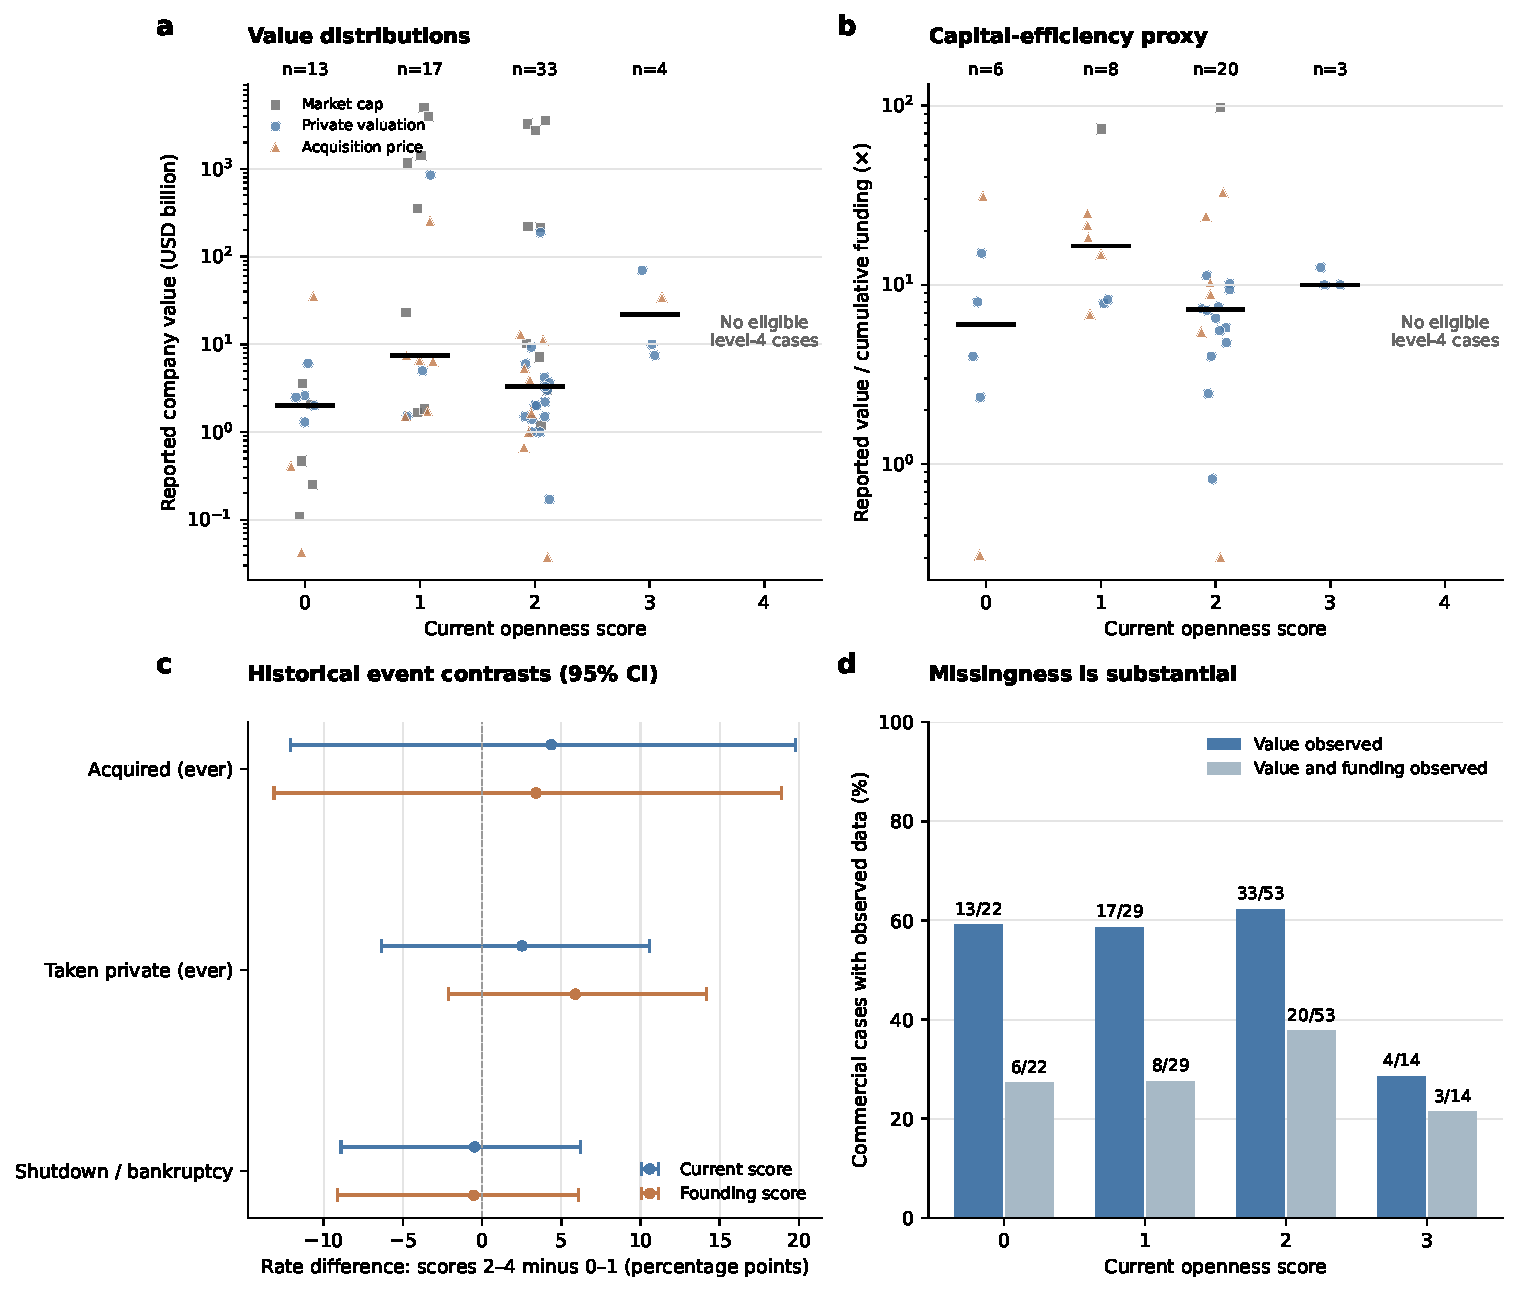
\includegraphics[width=\textwidth]{../figures/investment_evidence.pdf}
\caption{Observed values, capital-efficiency proxies, historical event contrasts and missingness for commercial non-model entities. Black bars show medians. Event contrasts compare scores 2--4 with 0--1 and use Newcombe--Wilson 95\% intervals. No current level-4 entity qualifies. Execution \texttt{95ddb5a0-c3c5-438f-8083-cacf439a71f0}; supplied exports, recomputed in \texttt{analysis.py}.}
\label{fig:overview}
\end{figure}

\subsection{How much bias can I
quantify?}\label{how-much-bias-can-i-quantify}

\textbf{Failure selection dominates.} One shutdown and one bankruptcy in
118 selected commercial entities cannot estimate venture mortality. A
functioning acquired brand, an absorbed company and shareholder loss are
different endpoints. The list includes distressed acquired hardware
brands without coding them as shutdowns. I will not import an external
``typical failure rate'' and pretend it calibrates this sample.

A simple omission stress test shows the fragility: with no missing
successes, adding \textbf{seven omitted failures} to the currently open
group changes its failure fraction from 1/67 to 8/74 = 10.8\%; adding
\textbf{five} to the restricted group changes 1/51 to 6/56 = 10.7\%. To
reach 25\% would require 21 and 16 omitted failures respectively. These
are scenarios, not estimates of how many are actually missing. Actual
relative failure risks are unidentified without the sampling frame.

\textbf{Outcome disclosure is selective.} Funding is absent in
\textbf{112/179 (62.6\%)} rows. Among the 118 commercial entities, 63
have recorded funding (62 positive), 67 have valid values, and only
\textbf{37/118 (31.4\%)} have a usable proxy. For current scores 2-4
versus 0-1, value coverage is \textbf{37/67 (55.2\%) versus 30/51
(58.8\%)} and proxy coverage \textbf{23/67 (34.3\%) versus 14/51
(27.5\%)}. For strictly current score 3, value coverage falls to
\textbf{4/14 (28.6\%)}, versus 63/104 (60.6\%) below 3. More than half
of each primary group's proxies are missing, so their full-sample median
ordering cannot be bounded without assumptions about the missing cases.
Missing funding is not zero funding.

As a deliberately extreme missing-value stress scenario, labeling every
commercial entity without a value as failed would give 44.8\% for
current scores 2-4 and 41.2\% for 0-1, instead of 1.5\% and 2.0\%. Many
are operating companies, so that scenario is not a plausible mortality
estimate. It demonstrates that complete-case results leave large parts
of the portfolio unpriced.

\textbf{Marks have different clocks.} Of 67 primary values, \textbf{21
(31.3\%) are more than two years old}, 17 exceed four years, and the
oldest is about 18.7 years old. The set mixes 27 private marks, 22
market caps and 18 acquisition prices. No inflation, liquidity or risk
adjustment can make those shareholder proceeds without underlying
financing histories. I preserve recorded values and disclose the
mismatch rather than invent a mark-down rule.

\textbf{Sector and claimant confounding are large.} The nine Big Tech
rows contribute nine values and zero usable funding multiples. The top
five companies supply \textbf{78.8\%} of the approximately USD 23.69
trillion commercial value sum. Foundation/government/nonprofit outcomes
are not observations of venture-equity capture. Open-model releases are
not independent founding-company treatments. Even within companies,
current score can follow success, distress, funding or acquisition;
measuring it after the outcome creates reverse causality. Initial scores
help with ordering but not selection or inconsistent historical
definitions.

\textbf{Search and scoring bias are visible but not correctable.}
Exactly \textbf{150/179 rows} have the literal search-tool label
``WebFetch (search budget exhausted),'' and six have no search-tool
label; others include mixed search/fetch descriptions. That is uneven
ascertainment, not proof those entries are wrong. The rubric is
unblinded and spans incompatible bundles of rights across industries. It
grants governance a score increment while companies are judged on
proprietary revenue-generating features. There is no inclusion
probability, independent score adjudication or complete failed-company
roster, so inverse-probability weighting, causal matching and a credible
survival curve are not available.

The all-179-row and expanded definitions, per-level rate intervals, full
sector-by-score cross-tabs, confidence flags, event timing and
concentration calculations remain available in the reproducibility
tables. They are not hidden by the primary filter.

\section{Ten investment concerns, ranked by
severity}\label{ten-investment-concerns-ranked-by-severity}

The order is my investment judgment for an alloy-discovery spin-out, not
a statistical risk score. ``For'' means evidence supporting the concern;
``against'' means the strongest counterevidence I can find in the
supplied record or verified sources. A counterargument is not a
validated company result.

\subsection{The company may fund a public good that competitors monetize
--
critical}\label{the-company-may-fund-a-public-good-that-competitors-monetize-critical}

\textbf{For:} The proposal releases methods, drivers,
composition/process records and failed runs, generally within 12 months.
It also defaults to publishing compositions. A buyer could use the
outputs without paying the producer. The claimed USD 8.8 trillion
benefit goes to users; the dataset has no dependable capture premium.
\citep{Hoffmann2024Value,InputProposal}

\textbf{Against:} Red Hat's recorded USD 34 billion acquisition,
Databricks' USD 190 billion private mark and several profitable-looking
company-value/funding proxies show that openness is compatible with
large enterprise value. Physical production, trusted validation,
proprietary customer workflows and service-level guarantees may remain
scarce. The dataset does not measure those mechanisms.

\textbf{IC judgment:} I need a specific reason a customer repeatedly
pays \emph{this} company after the relevant code and data become public.
``Open core plus services'' is a label, not an answer. Selling qualified
materials performance is potentially stronger than selling access to the
same information everyone receives.

\subsection{Academic demand may not become an industrial purchasing
budget --
critical}\label{academic-demand-may-not-become-an-industrial-purchasing-budget-critical}

\textbf{For:} The concrete commercialization example is a small
educational kit with USD 2.24 stated profit. There are no supplied
signed industrial orders, renewal cohorts, pricing experiments, sales
pipeline conversion or willingness-to-pay measurements. Science
marketing by AI providers is not customer demand for this spin-out.
\citep{InputBrief,InputRecommendations}

\textbf{Against:} The dataset contains commercial lab and
scientific-software firms, including Benchling and Schrodinger. Missing
APIs and integration difficulties indicate user pain. Openness may
reduce trials and procurement friction.

\textbf{IC judgment:} Pain and downloads are not budgets. I need paid
orders from the people responsible for yield, certification, production
cost or product development, not just researchers accepting subsidized
access. A service business selling low-volume university integrations
may be viable without meeting venture return requirements.

\subsection{Autonomous discovery may not transfer into reproducible,
manufacturable alloys --
critical}\label{autonomous-discovery-may-not-transfer-into-reproducible-manufacturable-alloys-critical}

\textbf{For:} The documents contain no customer-linked evidence of
repeatable alloy properties across builds, batches or laboratories; no
uncertainty-calibrated comparison against skilled human design; and no
demonstrated transfer from screening scale to qualified manufacturing.
General AlphaFold and patent-citation evidence does not supply these
results. \citep{InputBrief,Bryan2021,InputProposal}

\textbf{Against:} Public materials databases and open optimization tools
are useful inputs. Releasing provenance and failed runs can expose
errors and improve reproducibility. The proposed digital thread is a
sound measurement foundation.

\textbf{IC judgment:} Novel composition count is the wrong milestone. I
want independently verified property/process improvements at the
customer's relevant manufacturing conditions, including repeatability,
failure modes and cost. The actual bottleneck may be characterization or
qualification rather than composition search.

\subsection{Integration and support may consume the gross margin -- very
high}\label{integration-and-support-may-consume-the-gross-margin-very-high}

\textbf{For:} Only about 4/20 instruments reportedly expose usable
programmable interfaces, and the strategy includes wrapping closed
equipment and camera-reading interfaces. The hardware savings claim
excludes the full operating cost. Open drivers require continuing
validation after instrument and firmware updates.
\citep{InputRecommendations,Pearce2020}

\textbf{Against:} Reusable drivers and a shared schema could amortize
engineering across deployments. Documentation, warranties and managed
operation are services that customers can rationally pay for even when
designs are open. The hardware sample contains success cases as well as
distress.

\textbf{IC judgment:} I need a deployment-level contribution statement
after founder-equivalent labor, calibration, downtime, cloud/AI charges,
consumables, scrap, support and warranty reserves. Otherwise ``sell
services'' can mean selling scarce engineering hours at consulting
margins, with no scalable product leverage.

\subsection{Capital intensity and financing risk may erase attractive
technical outcomes -- very
high}\label{capital-intensity-and-financing-risk-may-erase-attractive-technical-outcomes-very-high}

\textbf{For:} Equipment, feedstock, process development and long
qualification cycles can require substantial capital before recurring
revenue. The dataset's Opentrons proxy is 0.83x and Markforged's
asset-price proxy 0.31x; Desktop Metal has a bankruptcy event. No cap
table, cash plan, debt schedule, plant utilization or subsequent-round
requirements are supplied. \citep{InputData}

\textbf{Against:} A university spin-out may access existing equipment
and grants rather than building a plant immediately. Contracting with
existing manufacturers could reduce asset intensity. Software-oriented
deployment could need less capital, but it is a different investee from
a foundry.

\textbf{IC judgment:} Grants are not free unless their obligations and
full economic costs fit the commercial model. I need cash to the next
value-creating milestone with an adequate delay reserve, and investor
returns after realistic future dilution. Large headline company values
are irrelevant if new capital captures the upside.

\subsection{The company may not own, or be able to license, what it
plans to sell -- very
high}\label{the-company-may-not-own-or-be-able-to-license-what-it-plans-to-sell-very-high}

\textbf{For:} The proposal flags inconsistent composition-IP positions
and an unresolved funded/unfunded Thermo-Calc relationship. It
references third-party databases, proprietary instrument documentation,
university ownership and grant-related sharing obligations. None of the
executed assignments, award terms, licenses, patent claims or
freedom-to-operate analysis is supplied. Public disclosure may be
irreversible. \citep{InputRecommendations,InputProposal}

\textbf{Against:} The draft recognizes these conflicts, proposes
third-party exclusions and calls for technology-transfer-office
agreement. Clear open licenses can reduce downstream uncertainty for
reusable code and attract adopters.

\textbf{IC judgment:} No investment before counsel signs off on chain of
title, the university's license to the spin-out, employee/inventor
obligations, foreground/background IP, grant rights and actual
data-derivative terms. A ``named prospective licensee'' is not an
exclusive license or an issued, enforceable patent. I will not
underwrite an assumption that an adapter or a provisional filing fixes
these issues.

\subsection{The OEM or AI platform may control the product's critical
path --
high}\label{the-oem-or-ai-platform-may-control-the-products-critical-path-high}

\textbf{For:} Closed SDKs, undocumented interfaces and
vendor-confidential manuals are recurring complaints. The
recommendations depend partly on an announced future hardware standard.
Vendors can change interfaces or terms; an AI platform can bundle the
driver layer. API wrappers alone may have low replacement cost.
\citep{InputBrief,InputRecommendations}

\textbf{Against:} Negotiated API/publication/export rights, modular
adapters and multiple compatible instruments can reduce lock-in. Neutral
protocols can make the company portable between AI providers and lower
customer resistance.

\textbf{IC judgment:} I need written commercial interface rights and a
tested fallback for every critical instrument and model provider. ``Open
standards will arrive'' is not a contingency plan. Do not confuse
control of a repository with control of laboratory access.

\subsection{Safety, qualification and liability may dominate the release
and revenue timetable --
high}\label{safety-qualification-and-liability-may-dominate-the-release-and-revenue-timetable-high}

\textbf{For:} Physical actuation, hot metal, powders, invalid sensor
readings and software-generated process settings create risks unlike a
database deployment. The kit's bill of materials and a general agent
protocol do not demonstrate safe closed-loop operation. Safety-critical
customer qualifications may outlast a 12-month publication embargo.
These are physical/contractual risks inferred from the proposed
application, not measured loss frequencies in the dataset.

\textbf{Against:} Transparent code, provenance and independent
inspection can help validation. Documented operating envelopes,
deterministic interlocks and an accountable operator could make
autonomous workflows safer and more auditable than ad hoc manual ones.

\textbf{IC judgment:} I require a hazard analysis, enforced interlocks
independent of the language model, calibrated uncertainty and stop
conditions, versioned validation, a human-accountability model,
appropriate insurance and a defined non-safety-critical beachhead. An
MCP server is not a safety certification.

\subsection{There may be no attractive exit for the actual business
built --
high}\label{there-may-be-no-attractive-exit-for-the-actual-business-built-high}

\textbf{For:} The brief borrows software IPO/acquisition medians for a
potential hardware-services/materials venture. The closest category has
zero usable financial multiples, the broader group only four.
Acquisition events include absorption, partial sales, distressed
outcomes and transactions without disclosed prices. A take-private is
not automatically a win. \citep{InputData,Boysel2025State}

\textbf{Against:} Strategic buyers do acquire scientific software,
hardware and open-source-origin vendors. Ansys, Red Hat and MakerBot
illustrate that different scientific/software/hardware assets can
attract buyers, although those historical deal records are not direct
alloy-lab comparables.

\textbf{IC judgment:} Show what a named class of buyer cannot
economically replicate or buy elsewhere, and why buying the company is
better than using the public releases, hiring the team or purchasing
instruments. Fund size, entry valuation and achievable ownership matter;
a good small business may still be the wrong fund investment.

\subsection{Governance and maintenance obligations may exceed the
spin-out's capacity --
material}\label{governance-and-maintenance-obligations-may-exceed-the-spin-outs-capacity-material}

\textbf{For:} The recommendations favor permissive release, public
working and eventual neutral governance while also claiming control of
the driver layer. There is no funded maintenance obligation, external
maintainer base, succession plan or commercialization management record
in the attachments. The asserted concentration of open-source value in a
few developers illustrates dependency risk, not free labor. Public
operation also needs credentials, security and customer-confidentiality
controls. \citep{InputRecommendations,Hoffmann2024Value}

\textbf{Against:} Open governance and upstream contributions can reduce
dependency on a single university lab, increase trust and allow
continuity if the company changes strategy. The existing public record
and license-audit activity are useful execution signals.

\textbf{IC judgment:} Set explicit boundaries: what the community
governs, what the board governs, who maintains safety-critical
integrations, what support is paid and what happens if grant support
stops. External contributors are a possible benefit, not a substitute
for a staffed operating budget.

\section{What would change my
assessment?}\label{what-would-change-my-assessment}

I would move from ``do not approve on this evidence'' toward investment
only after the following deliverables. The numerical gates below are
\textbf{my proposed underwriting thresholds}, not empirical conclusions
from the casebook; they should be adjusted to the eventual product and
fund economics.

\begin{enumerate}
\def\labelenumi{\arabic{enumi}.}
\tightlist
\item
  \textbf{A defined, tested product thesis.} Choose one primary model:
  qualified-alloy IP, production/discovery services, or a repeatable
  automation product. Identify the budget owner, use case, competing
  option and a narrow initial market. Show why legal public release does
  not remove the customer's reason to pay. I would reject a plan that
  silently needs exclusivity it has promised away.
\item
  \textbf{Paid, non-subsidized demand.} At least three independent
  industrial customers paying cash for representative pilots; at least
  two reorder, renew or contract for the next phase after receiving
  results. Disclose discounts, grants, university affiliation and
  founder labor. A letter of interest is insufficient. As a
  counterfactual, measure whether the same buyer would pay for the
  managed service after receiving the open deliverables.
\item
  \textbf{Blinded physical validation.} At least two independently run
  build/validation campaigns using customer-relevant material/process
  conditions, with a prespecified property/cost target, held-out
  compositions, complete failures and a credible baseline. Demonstrate
  repeatability across batches and an independent site or production
  partner. A dry software benchmark cannot substitute.
\item
  \textbf{Measured automation reliability and economics.} For the chosen
  workflow, initially demonstrate at least 100 consecutive
  representative attempted cycles with all interventions, failures,
  consumables, time and rework logged; report the denominator, not
  selected successful runs. Provide a credible scale-up validation plan
  beyond this small starting test. I would seek contribution margin of
  at least 40\% for a managed service or 60\% for a software-led product
  \emph{after} fully costing direct support and founder replacement,
  unless unusually strong retention or a different value proposition
  justifies less. These are screening gates, not claims that a
  particular margin guarantees venture scale.
\item
  \textbf{A signed rights package before public commitments.}
  Counsel-reviewed university license/assignments, grant and publication
  obligations, customer-data policy, vendor API/publication rights,
  patent strategy and freedom-to-operate risk register. Separate
  genuinely public funded outputs from customer-funded confidential work
  only where legally permitted. Do not assume an award can be
  renegotiated after taking the money.
\item
  \textbf{A financing and exit model I can audit.} Equipment
  ownership/lease terms, a cash budget through the next technical and
  commercial milestone plus a meaningful delay contingency, bottoms-up
  pipeline, hiring and support costs, future-round dilution, downside
  sale values, preferences and net investor proceeds. Show plausible
  fund-level returns at the proposed entry valuation in a base case, not
  just a software-multiple bull case. Compare outsourcing capital-heavy
  steps with owning them.
\item
  \textbf{A better evidence base for the openness decision.} A
  preregistered cohort of all relevant physical-science startups,
  including failed and never-funded firms; independent dimension-level
  scores for methods, hardware, data, compositions and governance; dated
  funding/cap tables and actual equity proceeds; age/sector/cohort-aware
  comparisons. Within the company, compare open-led versus other
  customer acquisition channels on qualified pipeline, conversion,
  acquisition cost, retention and contribution profit. Repository stars
  alone would not move me.
\end{enumerate}

\textbf{Evidence that would make me more negative:} customers use the
releases but will not pay for service; every installation requires
extensive new bespoke work; repeat property gains disappear on
independent fabrication; a vendor can block commercial operation;
ownership or data licenses cannot be cleared; or financing depends on
repeatedly marking up a capital-intensive service business at software
multiples.

\textbf{Bottom line:} I would retain openness where it demonstrably
lowers distribution cost, improves reproducibility or unlocks
procurement. I would not pay a premium for it as a moral attribute or a
surrogate for defensibility. If the primary objective is durable public
infrastructure, grants, philanthropy or a service-oriented sustainable
business may be a better capital structure than venture equity. That is
a financing judgment, not a judgment against open science.

\section{Discretionary analytical
decisions}\label{discretionary-analytical-decisions}

\begin{itemize}
\tightlist
\item
  \textbf{Commercial units first, raw sample retained.} I exclude model
  releases and institutional public goods from the primary investment
  comparison because their rights and economic claimants differ. I
  retain all-179-row and 133-row expanded analyses so this choice is
  inspectable.
\item
  \textbf{No invented values.} I use only the three explicit valuation
  types, never revenue/grants as value, missing funding as zero or zero
  funding as an infinite multiple. I label the Desktop Metal
  zero-recovery test as a scenario.
\item
  \textbf{Founding and current scores analyzed separately.} I do not
  infer the timing or effect of licensing from a cross-sectional current
  score. I show score-by-score results, a 2-4 versus 0-1 contrast and a
  stricter threshold at 3 because the economic distinction is
  contestable.
\item
  \textbf{Medians, distributions and resampling rather than summed
  ``success.''} Extreme concentration and mixed marks make aggregate
  value a poor outcome; I show IQRs, full observations, sample sizes and
  conditional uncertainty. A one-case group does not receive a spurious
  financial CI.
\item
  \textbf{Historical events, not survival claims.} I distinguish
  acquisitions, take-privates, shutdowns and bankruptcies, count
  organizations rather than repeated transactions and retain overlapping
  outcomes. I do not fit a survival curve without a complete risk set
  and ascertainment history.
\item
  \textbf{Simple, exploratory adjustment and explicit sensitivities.}
  Sector/cohort controls, mark-type controls, recency, confidence,
  threshold and impairment checks expose instability. I do not interpret
  noisy, selected subgroups or uncorrected p-values as discoveries, nor
  claim that wide intervals prove equivalence.
\item
  \textbf{Risk ranking and gates are investor judgments.} I prioritize
  appropriation, customer budgets and transferable physics over license
  ideology. Proposed customer, cycle and margin gates are disclosed
  decision rules, not scientific estimates.
\end{itemize}
